Ein Projektorganigramm ist ein wichtiges Instrument zur Darstellung der internen Struktur und der wechselseitigen Beziehungen innerhalb eines Projektteams. Es ermöglicht einen klaren Überblick über die verschiedenen Rollen und Verantwortlichkeiten der Mitarbeiter, sowie deren Hierarchieebenen und deren jeweilige Berichtswege \cite{projektmanagement-definitionen:2009}.

\begin{figure}[H]
	\centering
	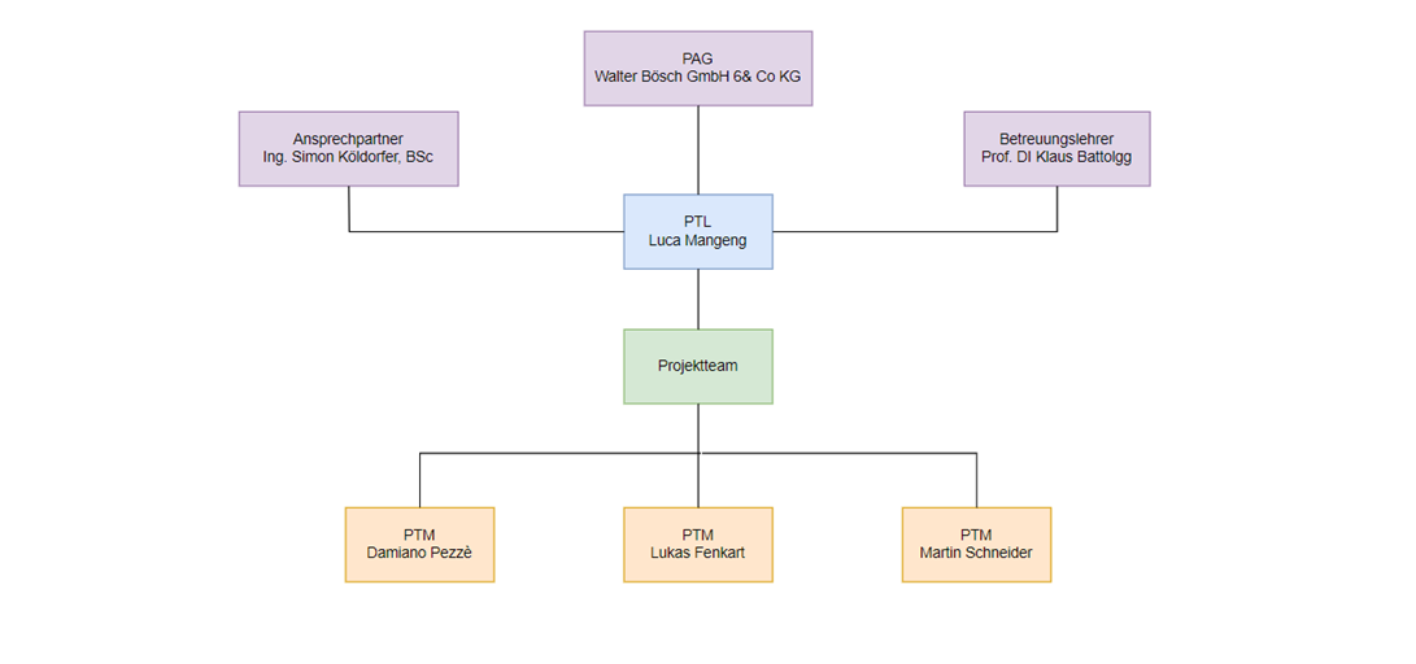
\includegraphics[width=0.9\linewidth]{Bilder/Organigramm}
	\caption{Projektorganigramm}
	\label{fig:organigramm}
\end{figure}

\begin{table}[H]
	\caption{Projektorganisation}
	\label{tab:projektorganisation}
	\begin{tabular}{p{\dimexpr 0.25\textwidth-2\tabcolsep} | p{0.50\textwidth} | p{0.20\textwidth}}
		\toprule
		\textbf{Projektrolle} & \textbf{Aufgabenbereich/Skills} & \textbf{Name} \\
		\midrule
		Projektauftraggeber & Gibt den Auftrag für die Universalananzeige an und setzt Bedingungen und Ziele, die im Projekt erreicht werden sollen. Auch setzt er eine Fertigstellungsfrist & Walter Bösch GmbH und Co KG
		\\
		\midrule
		Projektleiter & Leitung des Projekts;
		Verantwortlich für die Einhaltung der Fertigstellung des Projekts und für die Einhaltung der Bedingungen; Hilft bei der Programmierung, dem Aufbau der Hardware den Berechnungen und Tests
		 & Luca Mangeng
		\\
		\midrule
		Projektteam-mitglieder & Zuständig für die Erstellung des Codes, Zusammenstellung und Zusammenbau der preiseffizienten Hardware & 
		Lukas Fenkart, Damiano Pezzè, Martin Schneider
		\\
		\bottomrule
	\end{tabular}
\end{table}